\chapter{Experimenteller Aufbau}\label{cha:experimentAufbau}
\section{Versuchsanordnung}\label{sec:versuchsanordnung}

Wie bereits in \autoref{sec:versuchsTheorie} erläutert, basiert das Millikan-Experiment auf dem Kräftegleichgewicht zwischen der Gewichtskraft und der elektrischen Kraft. Zu Beginn wird ein dunkler Raum benötigt, wobei eine Dunkelkammer, in der keinerlei äußeres Licht eindringen kann, ideal ist. Das einzige Licht, das während des Experiments verwendet wird, stammt aus einem Mikroskop, das am Experimentapparat angebracht ist.

Während des Versuchs werden sehr kleine Öltröpfchen mithilfe eines Zerstäubers in eine Kammer eingebracht. Die Fallgeschwindigkeit der Tröpfchen wird anschließend durch Beobachtung mit dem Mikroskop und anhand des Lichts gemessen.

Die Kammerwände, sowohl der Boden als auch die Decke, bestehen aus elektrisch geladenen Kapazitoren, was es ermöglicht, ein elektrisches Feld zu erzeugen. Über einen Schalter kann die Richtung des elektrischen Feldes verändert werden. Diese Funktion wird insbesondere bei der zweiten Messung benötigt, bei der die Kapazitoren aktiviert werden, sodass das elektrische Feld nach oben gerichtet ist (Decke + Boden -). Wenn die Öltröpfchen negativ geladen sind, können sie die Gravitationskraft überwinden und steigen nach oben. Die Geschwindigkeit, die die Tröpfchen benötigen, um von einer Gitterlinie zur nächsten zu gelangen, wird dabei erneut gemessen. Dieser Vorgang wird wiederholt, bis das Tröpfchen nicht mehr sichtbar ist. Eine detaillierte Schritt-für-Schritt-Anleitung wird in \autoref{sec:durchfuehrung} bereitgestellt.

\section{Material}\label{sec:material}

In dieser Arbeit wurde das \textit{Model AP-8210 von PASCO scientific} mit der Halogenlampe verwendet. \\

\noindent \textbf{Material, das dabei ist:}

\begin{itemize}
	\item Apparat Plattform und Kondensator Ladungsschalter (Eine genauere Beschreibung der Plattform in \autoref{sub:inhaltApparatur})
	\item 12 Volt DC Transformator für die Halogen Lampe
	\item nicht flüchtiges Öl
	\item Ölsprüher 
\end{itemize}

\subsection{Plattform}\label{sub:inhaltApparatur}
Da das Experiment bereits vollständig aufgebaut ist, werden im Folgenden alle Komponenten aufgezählt, die sich auf der Plattform befinden.

\noindent \textbf{Komponenten Plattform:}

\begin{itemize}\label{item:apparatur}
	\item Tröpfchenbetrachtungskammer (Wird im nächsten \autoref{sub:viewingChamber})
	\item Betrachtungsfernrohr (30X, Hellfeld, aufrechtes Bild) mit Fadenkreuz (Linienabstand: 0,5 mm große Teilung, 0,1 mm kleine Teilung), Fadenkreuz-Fokussierring und Tropfenfokussierring
	\item Halogen Lampe (12 V, 5 W)
	\item Fokussierdraht
	\item Kondensatorenspannungs Anschlüsse
	\item Thermistor Anschlüsse (sind an den unteren Kondensator eingebaut)
	\item Thermistor Tabelle (Widerstand-Temperatur)
	\item Ionisationsquellen Schalter (3 verschiedene Positionen: Ionisation AN, Ionisation AUS, Sprüh Position)
	\item Wasserwaage
	\item Kondensator Ladungsschalter (mit einem Meter Kabel, um Vibrationen aus dem Weg zu gehen)
\end{itemize}


\subsection{Betrachtungskammer}\label{sub:viewingChamber}
Die Betrachtungskammer ist zerlegbar. Die einzelnen Komponenten werden im Folgenden aufgelistet.

\noindent \textbf{Einzelteile der Betrachtungskammer:}

\begin{itemize}\label{item:betrachtungskammer}
	\item Deckel
	\item Gehäuse
	\item Tröpfchenlochabdeckung
	\item obere Kondensatorplatte
	\item Abstandshalter aus Plastik (ungefähr 7.6mm dick)
	\item untere Kondensatorplatte
	\begin{itemize}
		\item Thorium-232 Alphateilchenquelle
		\item elektronische Verbindung zur oberen Platte
	\end{itemize}
	\item konvexe Linse
\end{itemize}

\begin{figure}[h]
	\centering
	\begin{minipage}[t]{0.45\textwidth}
		\centering
		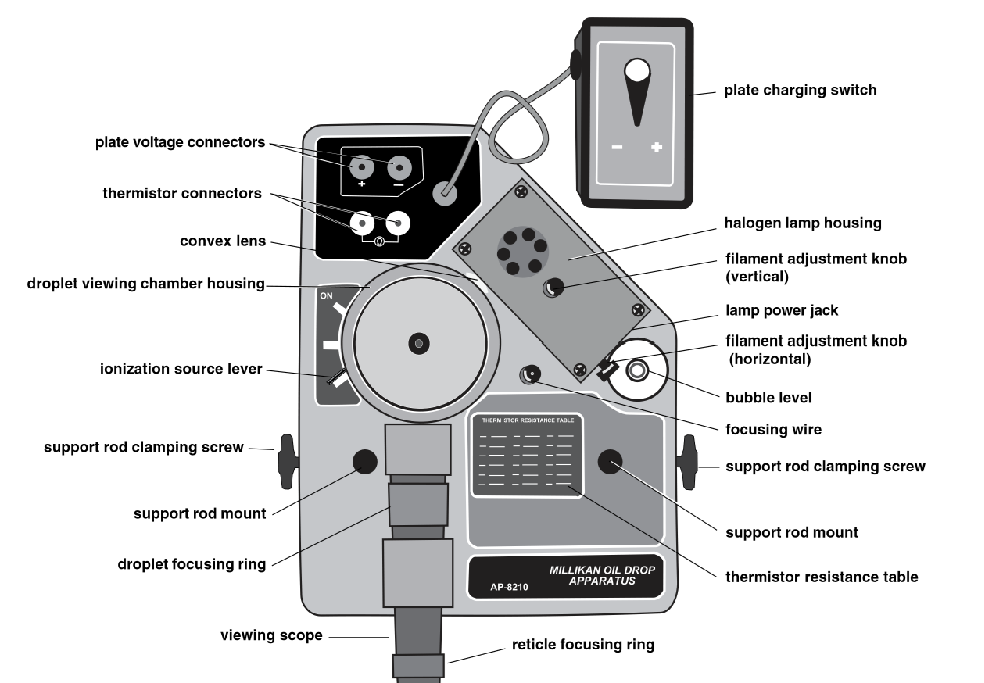
\includegraphics[scale=0.5]{bilder/pdf/plattformKomponenten.pdf}
		\caption{Komponenten der Plattform}
		\label{fig:plattformKomp}
	\end{minipage}
	\hfill
	\begin{minipage}[t]{0.45\textwidth}
		\centering
		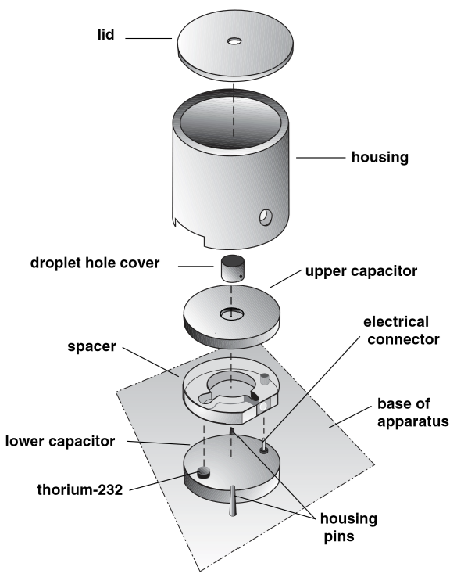
\includegraphics[width=\textwidth]{bilder/pdf/BetrachtungsKammerKomponenten.pdf}
		\caption{Komponenten der Betrachtungskammer}
		\label{fig:betrachtKomp}
	\end{minipage}
\end{figure}

\noindent Das gesamte Material ist in einem Experimentierkasten enthalten. Dieses Experiment wurde von der Kantonsschule am Burggraben für die Durchführung dieser Arbeit zur Verfügung gestellt.





